\documentclass[main]{subfiles}

\begin{document}
\begin{lect}
		\begin{example}
		    Экстремум кв. форму ны ед. сфере
				\[A = \begin{pmatrix}
					a_{11} & ... & a_{1n}\\
					...\\
					a_{n_1} & ... & a_{nn}
				\end{pmatrix} \qq a_{ij} = a_{ji}\]
				\[f : \R^n \to \R \qq f(x) = (Ax, x) = \sum^n_{i, j = 1} a_{ij} x_i x_j  \]
				\[\text{При условии } \sum^n_{j = 1} x_j^2 = 1 \]
				\[\Phi(x) = \sum^n_{j = 1} x^2_j - 1\]
				Если в т. $x^*$ - отн. экстремум, то
				\[\exists \lambda \in \R^n\]
				\[\begin{cases}
					\nabla f(x^*) - \lambda \nabla \Phi(x^*) = 0\\
					\Phi(x^*) = 0
				\end{cases}\]
				\[\nabla f = 2 A x\]
				\[\nabla \Phi = 2x\]
				\[\lambda \in \R\]
				\[\begin{cases}
					A x^* = \lambda x^*\\
					\sum x^{*2} = 1
				\end{cases} \Ra \lambda \text{ - с.ч. } \q x^* \text{ - с.в соотв. } \lambda\]
				\[\Abs{x^*} = 1\]
				\[A \begin{pmatrix}
					x_1\\
					\vdots\\
					x_n
				\end{pmatrix} =
			    \lambda \begin{pmatrix}
			    	x_1 \\
					\vdots\\
					x_n
			    \end{pmatrix}
				\]
				Ищем экстр. $f(x) = (Ax, x)$
				\[\Ra f(x^*) = (Ax^*, x^*) = (\lambda x^*, x^*) = \lambda \us{= 1}{(x^*, x^*)} = \lambda\]
				\[\Ra \max \text{ и } \min \text{ знач. кв. ф. на ед. сфере равны }\]
				\[\max \text{ и } \min \text{ с.ч. } A\]
		\end{example}

		\begin{Definition}
				\[L \in \LL(\R^n, \R^n) \qq (x, Ly) = (L^{*}x, y)\]
				\[\text{Норма } L : \q \Abs{L} = \max_{x \in S} \Abs{L_x} \]
				\[f(x) = \us{x \in S}{\Abs{Lx}}^2 = (Lx, Lx) = (L^{*}Lx, x)\]
				\[\Abs{L}^2 - \max \text{ с.ч. } (L^*L)\]
		\end{Definition}

		\section{Теория функций компл. переменного}
		\begin{Reminder}
		    \[z = x + iy \in \CC \qq x, y \in \R\]
				\[i^2 = -1\]
				\[z_1 + z_2 = x_1 + x_2 + i(y_1 + y_2)\]
				\[z_1 \cdot z_2 = x_1 x_2 - y_1 y_2 + i(x_1 y_2  + x_2 y_1)\]
				\[\overline{z} = x - iy \qq \abs{z} = \sqrt{x^2 + y^2}\]
	      \begin{figure}[H]
	        \centering
	        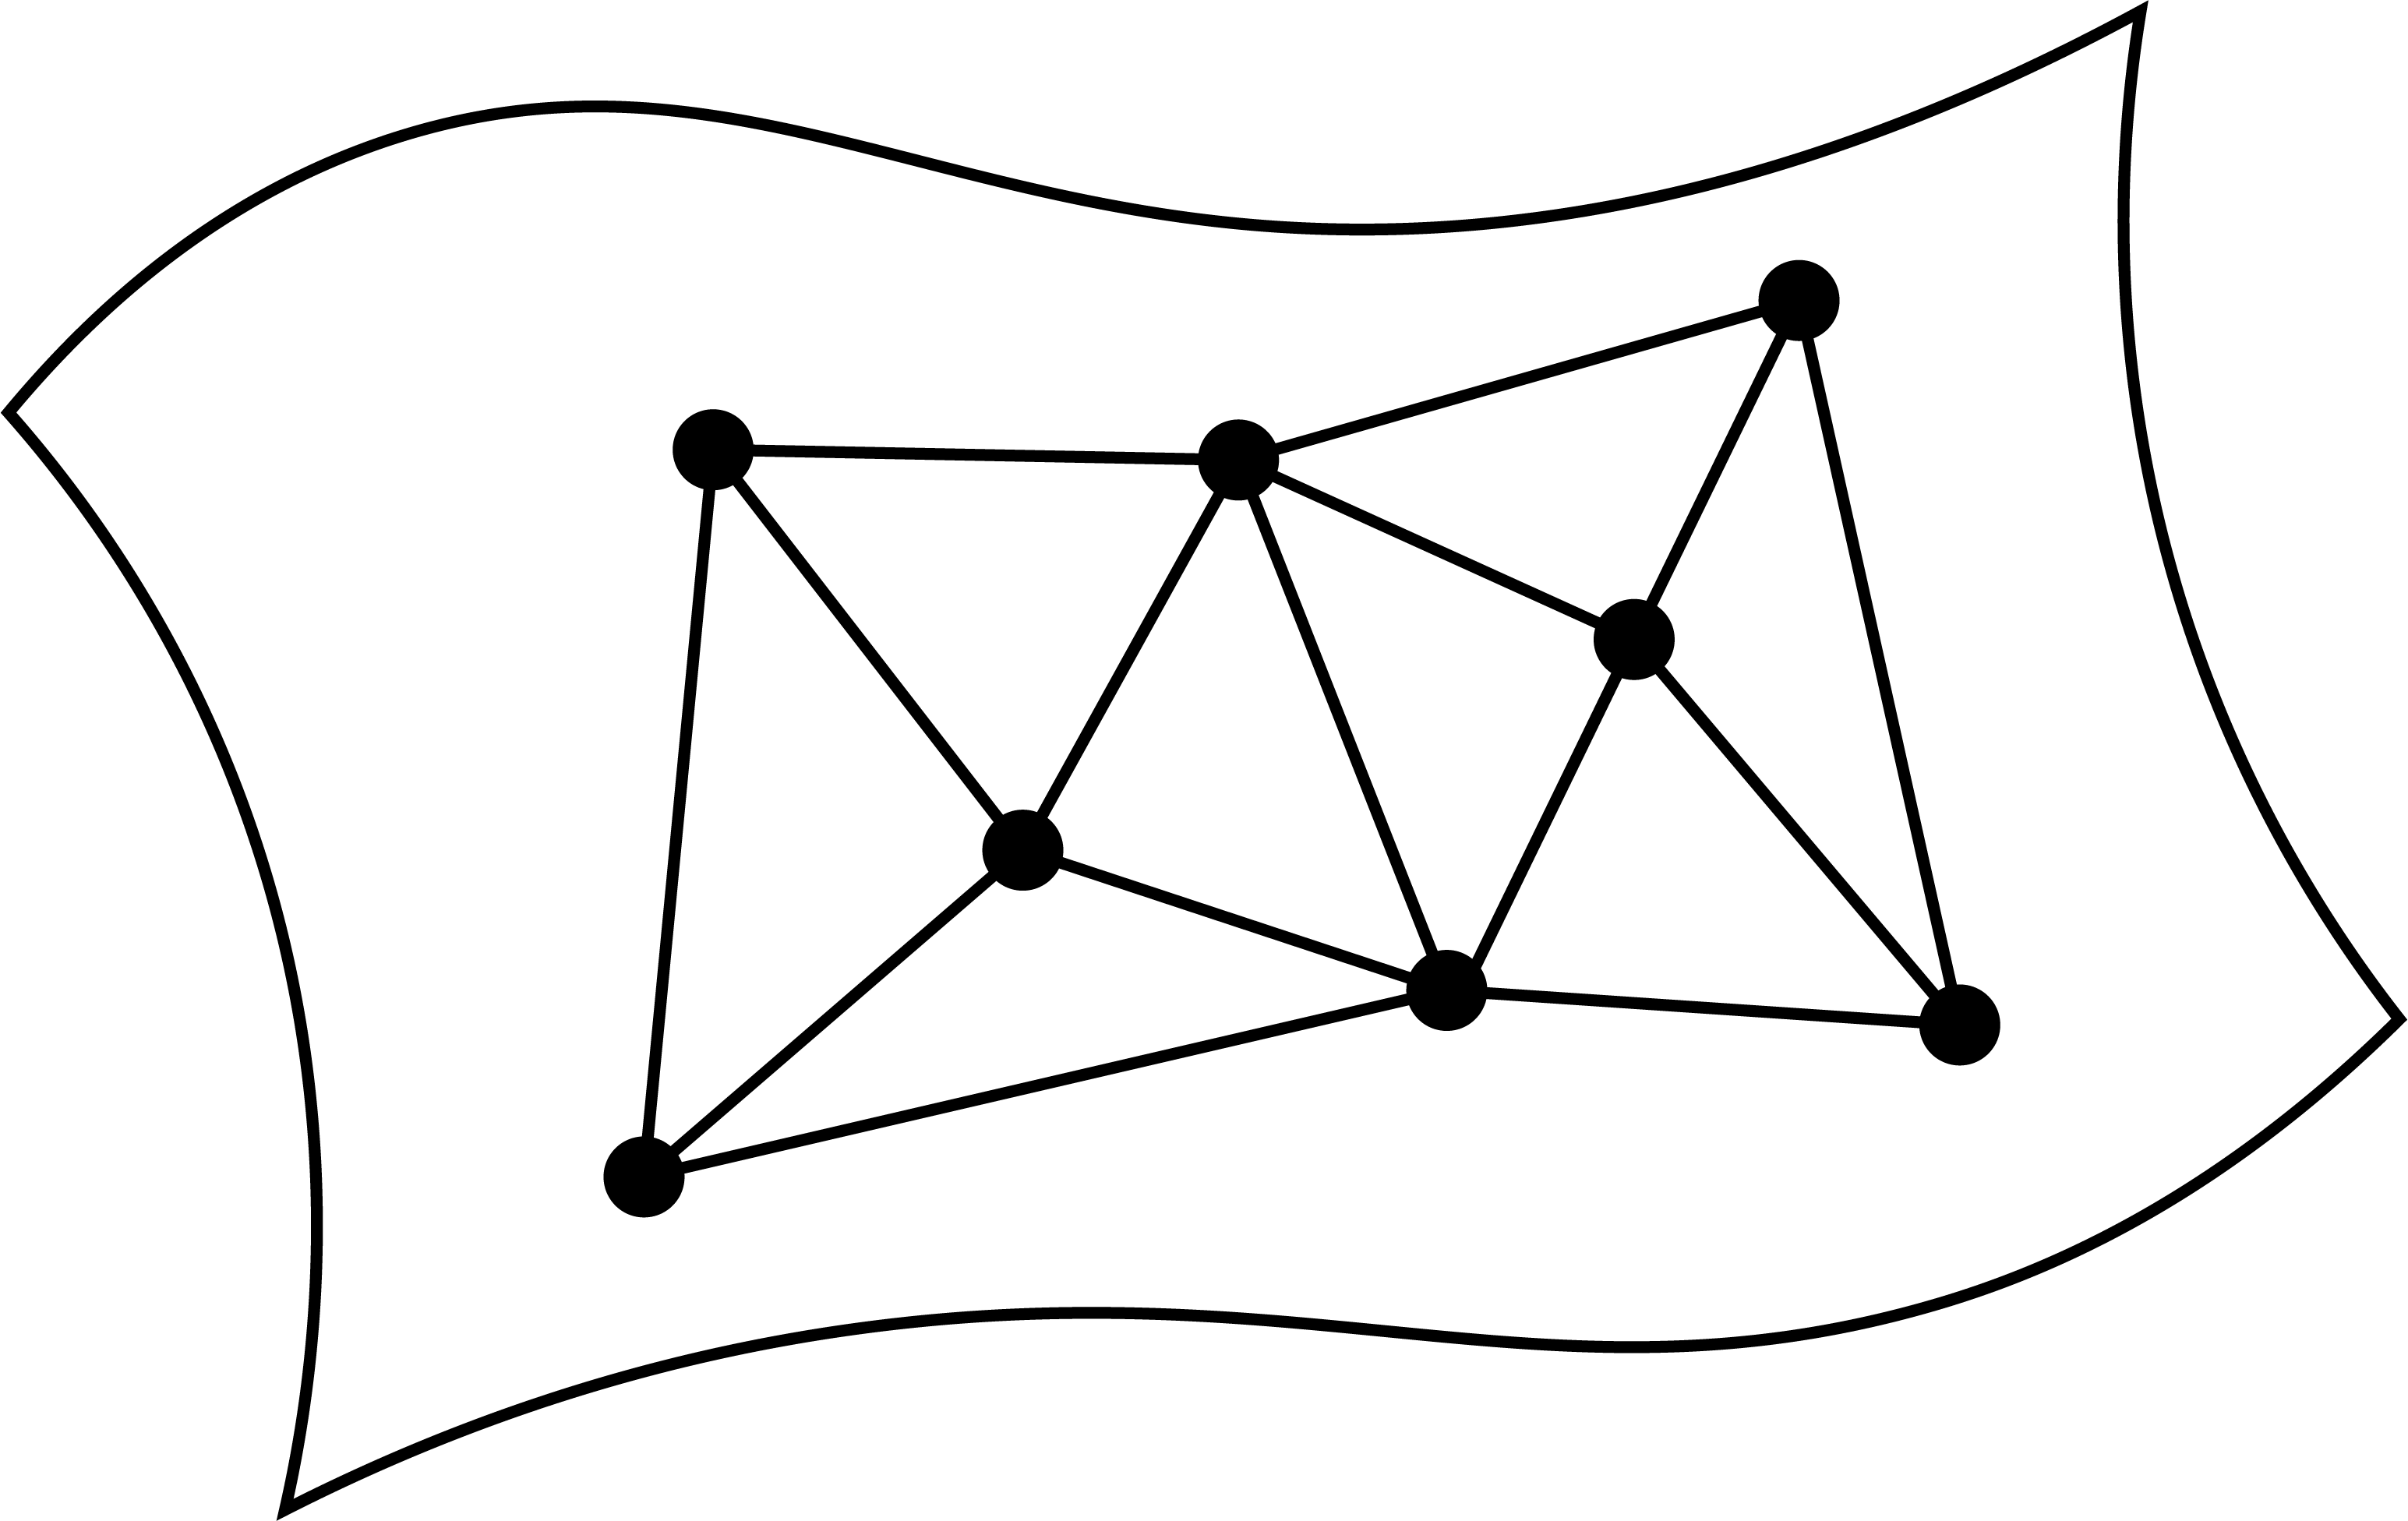
\includegraphics[width=5cm]{7_1}
	      \end{figure}
				\[z \cdot \overline{z} = \abs{z}^2\]
				\[\frac{z_1}{z_2} = \frac{z_1 \cdot \overline{z_2}}{\abs{z_2}^2}\]
				\[k \in \R \Ra \frac{z}{k} = \frac{x}{k} + i \frac{y}{k}\]
				Сложение действует как на векторах, что с умножением?\\
				Перейдем к полярной системе координат
	      \begin{figure}[H]
	        \centering
	        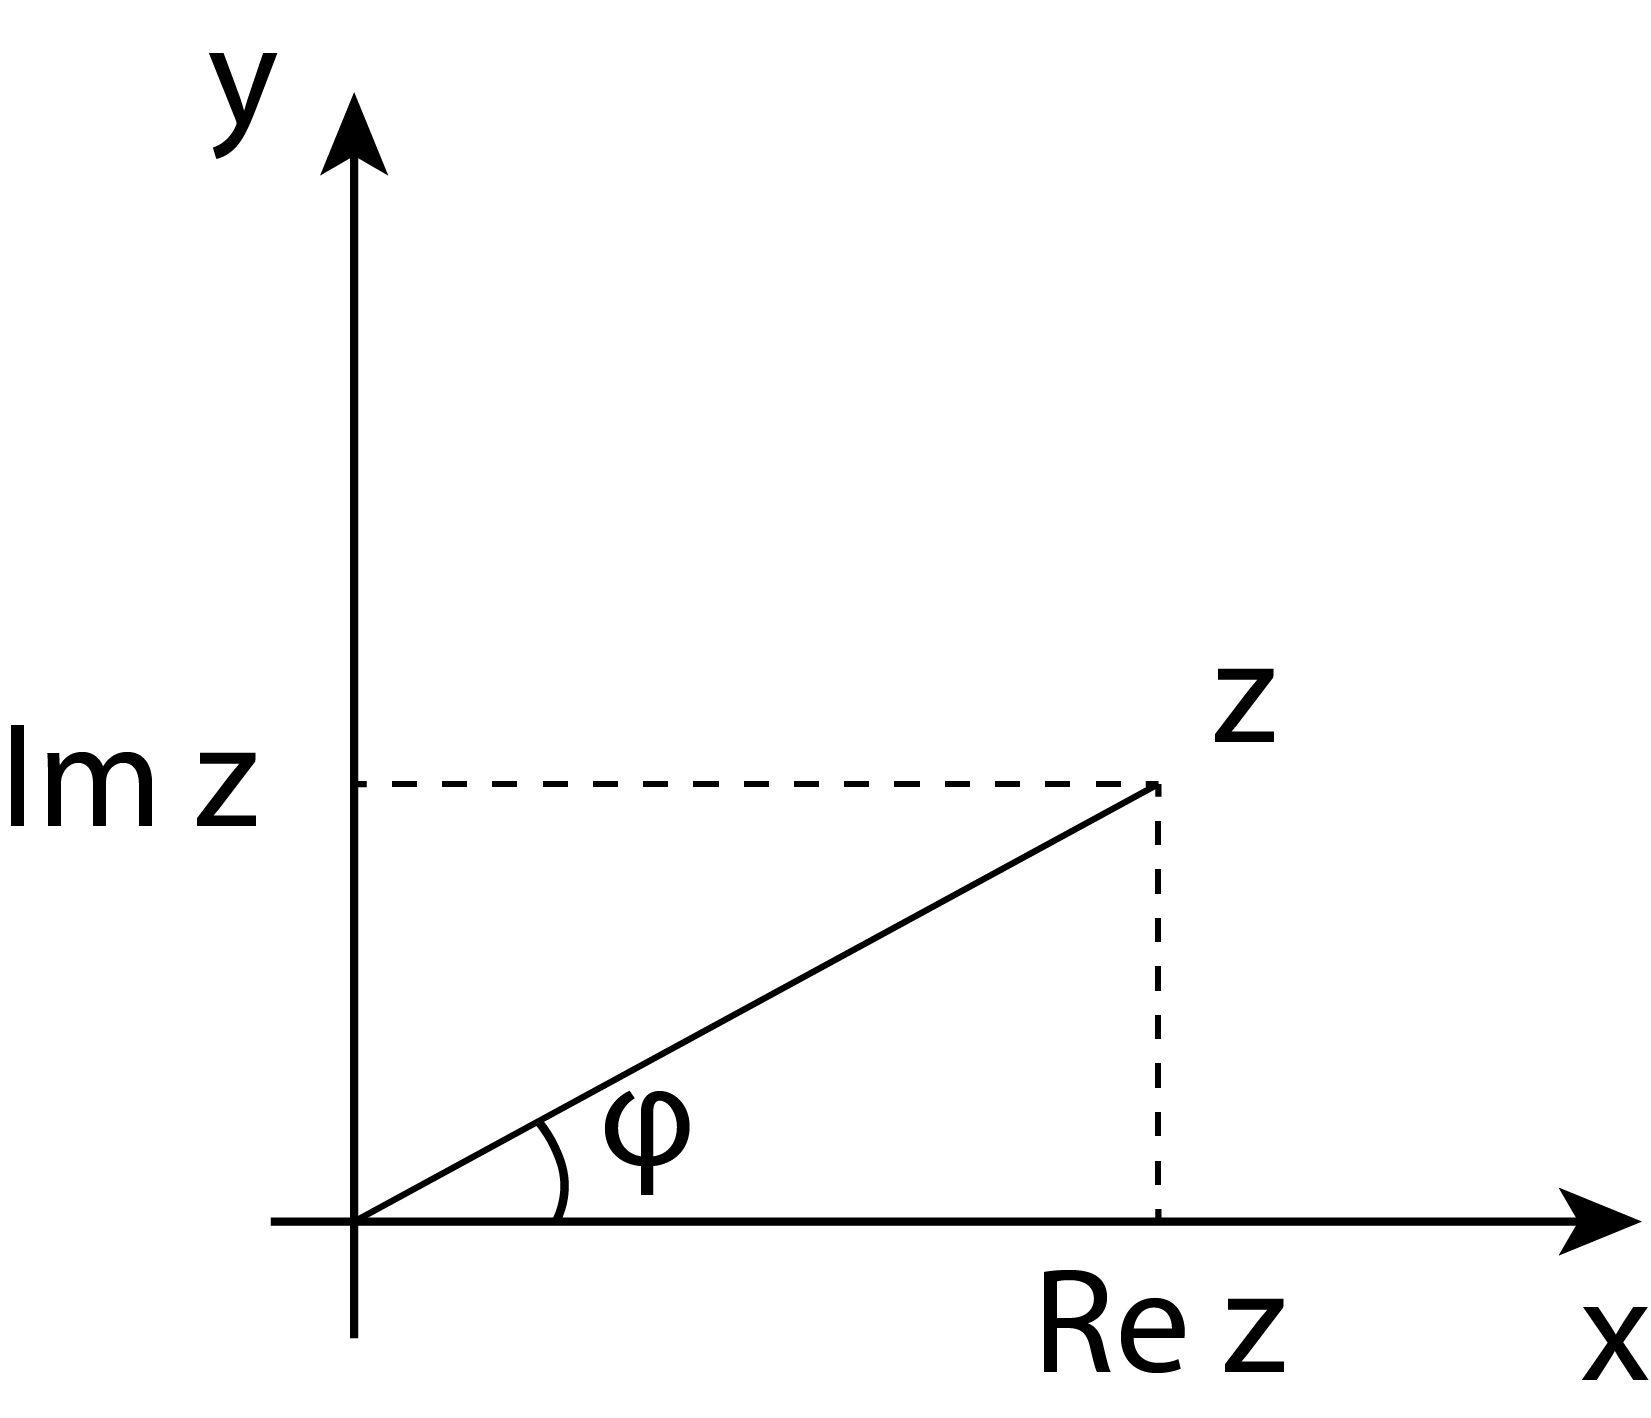
\includegraphics[width=5cm]{7_2}
	      \end{figure}
				\[z = \abs{z} (\cos \varphi + i \sin \varphi)\]
				\[\real z = \abs{z} \cos \varphi\]
				\[\im z = \abs{z} \sin \varphi\]
				\[z_1 = \abs{z_1} (\cos \varphi_1 + i \sin \varphi_1)\]
				\[z_2 = \abs{z_2} (\cos \varphi_2 + i \sin \varphi_2)\]
				\[z_1 \cdot z_2 = \abs{z_1} \cdot \abs{z_2}
				(\cos \varphi_1 \cos \varphi_2 - \sin \varphi_1 \sin \varphi_2
			    +i(\cos \varphi_1 \sin \varphi_2 + \sin \varphi_1 \cos \varphi_2)) = \]
				\[ = \abs{z_1} \abs{z_2} (\cos(\varphi_1 + \varphi_2) +
				i \sin (\varphi_1 + \varphi_2))\]
	      \begin{figure}[H]
	        \centering
	        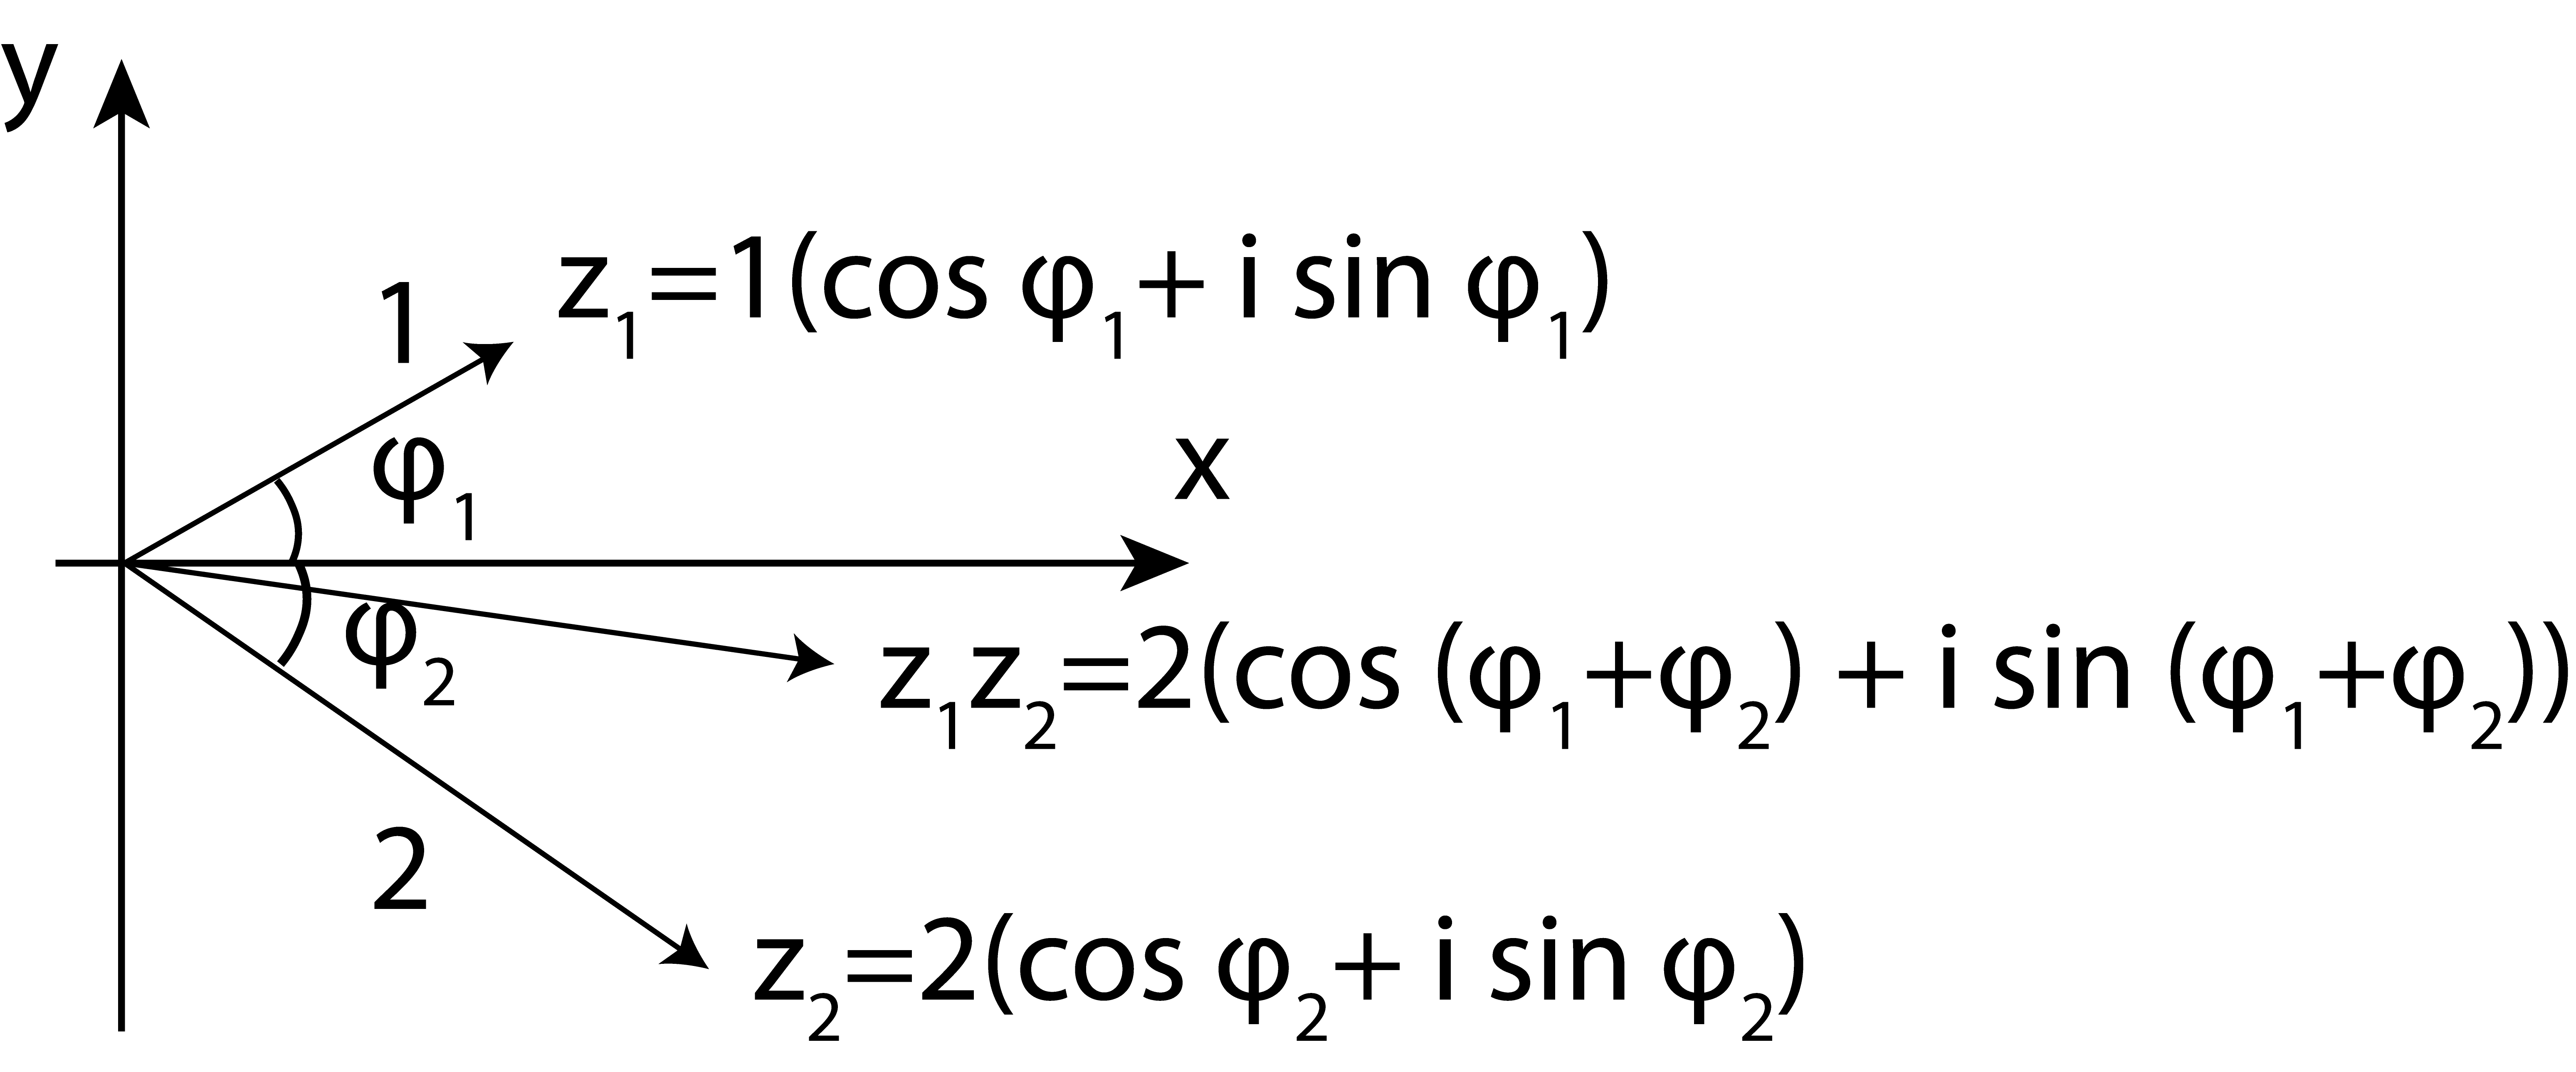
\includegraphics[width=7cm]{7_3}
	      \end{figure}
		\end{Reminder}

		\begin{Theorem} [Ф-ла Муавра]
				\[z^n = \abs{z}^n (\cos{n \varphi} + i \sin n \varphi )\]
		\end{Theorem}

		\begin{Definition} [н-во \bigtriangleup]
				\[\abs{z_1 + z_2} \leq \abs{z_1} + \abs{z_2}\]
		\end{Definition}

		\begin{Definition} [н-во Коши]
		    \[z_j, w_j \in \CC, \q j = 1, ..., n\]
				\[\abs{\sum_{j = 1}^n z_j \cdot w_j}^2 \leq \sum_{j = 1}^n
				\abs{z_j}^2 \cdot \sum_{j = 1}^n \abs{w_j}^2 \]
		\end{Definition}

		\begin{Proof}
				\[\overline{ab} = \overline{a} \cdot \overline{b} \qq
				z + \overline{z} = 2 \real z \qq
				z - \overline{z} = 2 i \im z\]
				%\[0 \leq \sum_{j = 1}^n  \abs{z_j - \lambda w_j}^2 =
				%\sum_{j = 1}^n  (z_j - \lambda w_j) (\overline{z}_j -
				%\overline{\lambda} \overline{w}_j) = \sum( \abs{z}^2 + \abs{\lambda}^2
			    %\abs{w_j}^2 - \]
				%\[- (z_j \overline{\lambda} w_j + \overline{z}_j \lambda w_j) ) =
				%\sum \abs{z_j}^2 + \sum \abs{\lambda}^2 \abs{w_j}^2 - \sum 2 \real
				%\underbrace{(\overline{\lambda} \cdot z_j \cdot w_j)}\]
				\[0 \leq \sum_{j = 1}^n  \abs{z_j - \lambda \overline{w}_j}^2 =
				\sum \abs{z_j}^2 + \abs{\lambda}^2 \sum \abs{w_j}^2 - 2 \real
			    (\sum_{j = 1}^n z_j \overline{\lambda} w_j)\]
				\[\lambda = \frac{\sum z_j w_j}{\sum \abs{w_j}^2}\]
				\[0 \leq \sum \abs{z_j}^2 + \frac{\abs{\sum z_j w_j}^2}
				{(\sum \abs{w_j}^2)^2} \cdot \sum \abs{w_j}^2 -
			    2 \real \left[  \frac{\sum \overline{z_j} \cdot \overline{w_j}}
		        {\sum \abs{w_j}^2} \sum_{j = 1}^n z_j w_j \right]\]
				\[\text{hint: } [...] \leq \frac{\abs{\sum z_j w_j}^2}{\sum \abs{w_j}^2}\]
				\[0 \leq \sum \abs{z_j}^2 + \frac{\abs{\sum z_j w_j}^2}{\sum \abs{w_j}} -
				2 \frac{\abs{\sum z_j w_j}^2}{\sum \abs{w_j}^2}\]
				\[\abs{\sum^n_{j = 1} z_j w_j}^2 \leq \sum^n_{j = 1} \abs{z_j}^2 \cdot
				\sum_{j = 1}^n \abs{w_j}^2 \]
		\end{Proof}

		\begin{definition}
		    Комплексная последовательность
				\[c_n \in \CC\]
				\[c_n = a_n + i b_n, a_n, b_n \in \R\]
				\[c_n \to c \in \CC \rla \abs{c_n - c} \to 0 \rla \begin{cases}
						a_n \to a\\
						b_n \to b
				\end{cases} \rla \{c_n\}_{n \in \N} \text{ - сх. в себе} \]
				\[\text{при } n \to \infty \qq \text{ т.е } \ \begin{align}
						\real c_n \to \real c\\
						\im c_n \to \im c
				\end{align}\]
		\end{definition}

		\begin{examples} [функций к. п.]
				\begin{enumerate}
						\item $ \us{\text{зафикс}}{a \in \CC}  \qq f(z) = z + a \qq f: \CC \to \CC$\\
							парал. перенос вдоль вектора $\overline{a} = (\real z, \im a)$
		          \begin{figure}[H]
		            \centering
		            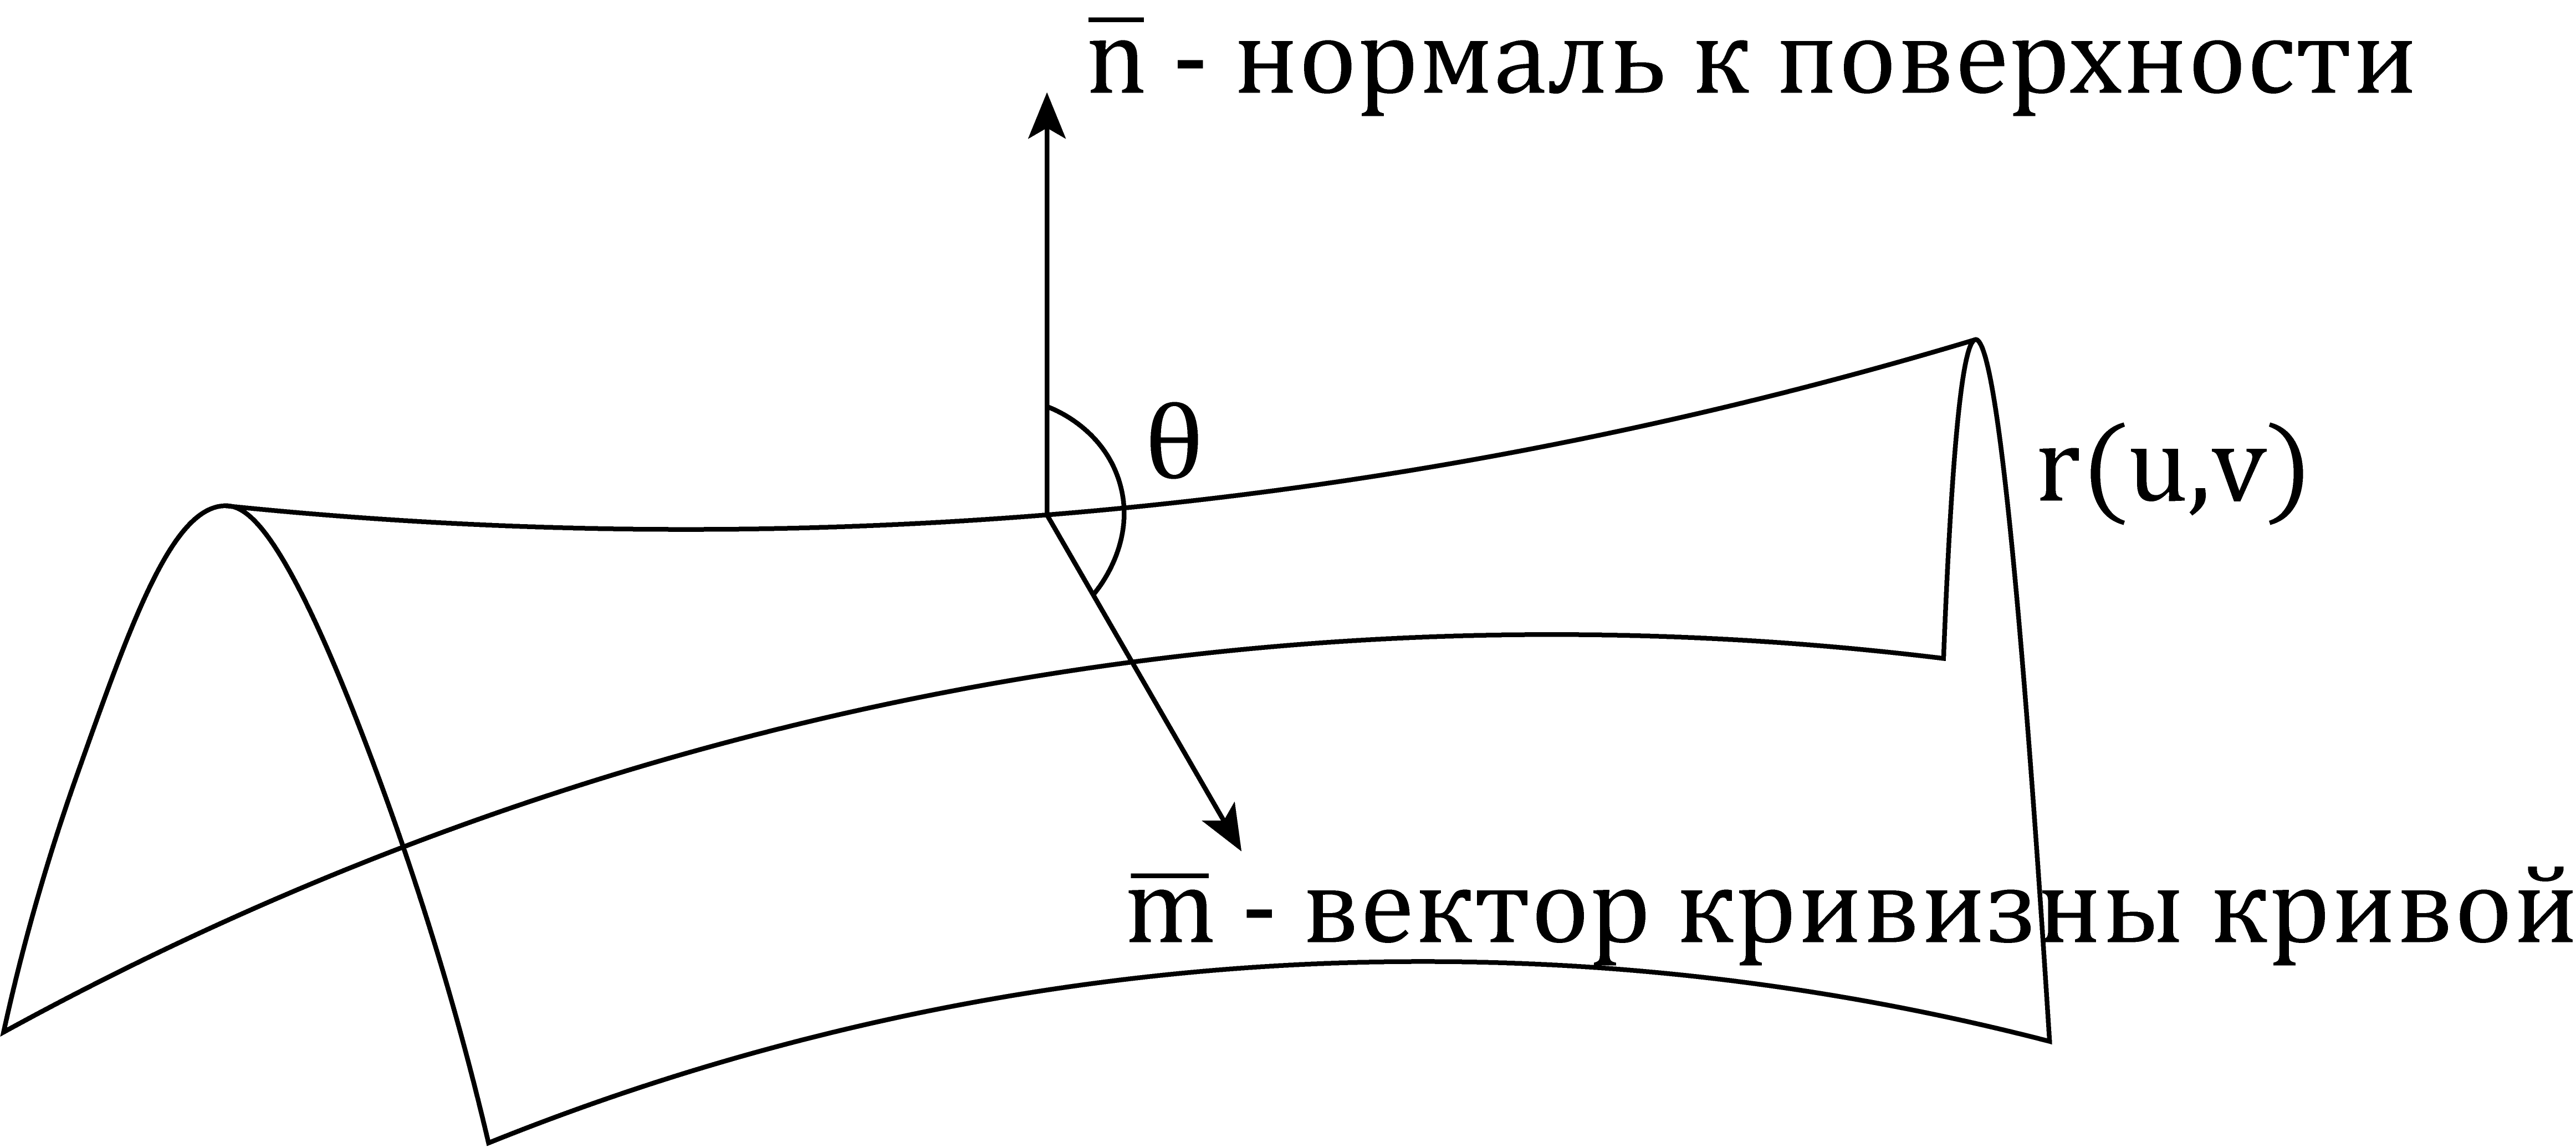
\includegraphics[width=5cm]{7_5}
		          \end{figure}
						\item $\lambda \in \CC \q \abs{\lambda} = 1 \q \lambda = \cos \Theta + i \sin \Theta \q
							z = \abs{z}(\cos \varphi + i \sin \varphi)$
							\[f(z) = \lambda z = \abs{z} (\cos(\varphi + \Theta) + i \sin (\varphi + \Theta))\]
							Поворот вокруг O на угол $\Theta$ против часовой стрелки
		          \begin{figure}[H]
		            \centering
		            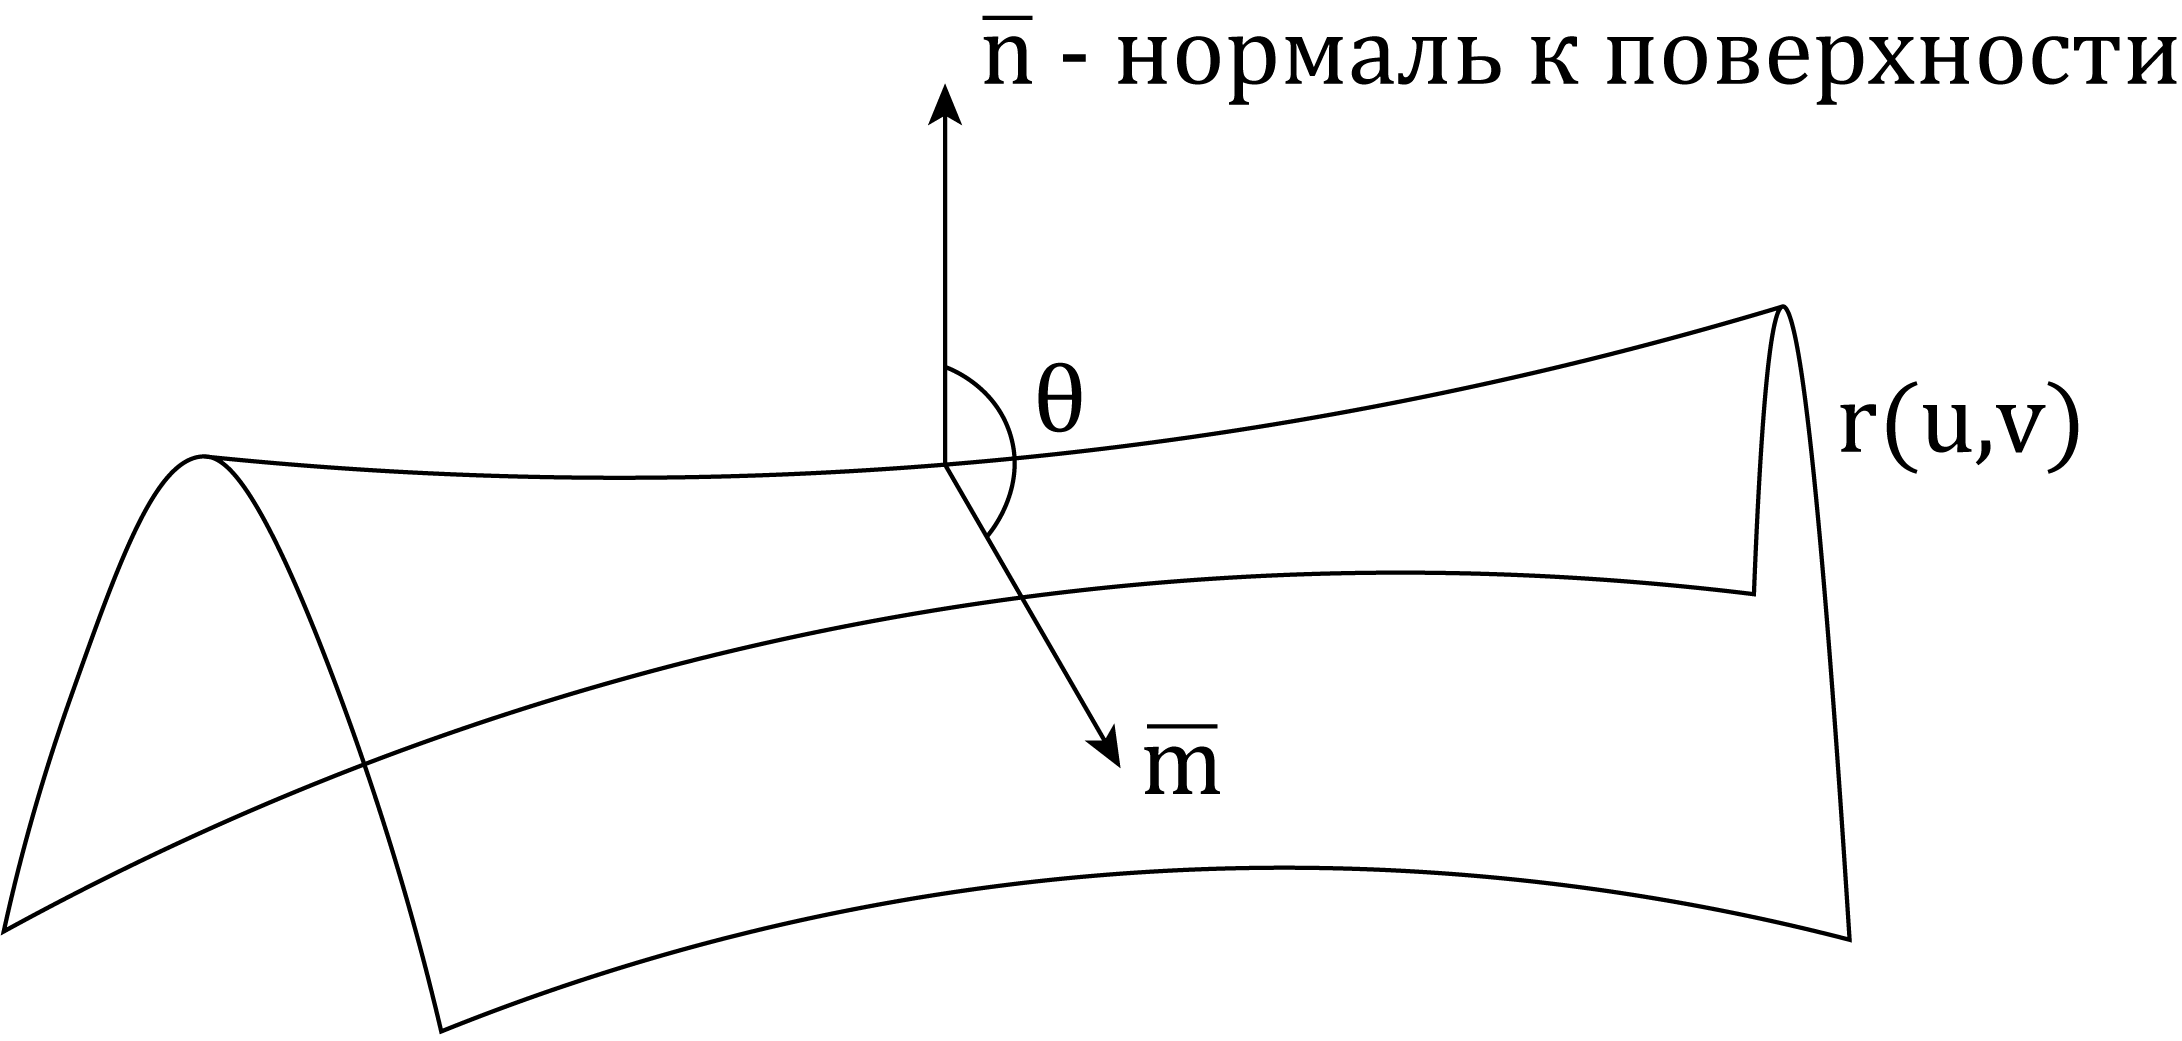
\includegraphics[width=5cm]{7_6}
		          \end{figure}
						\item $k \in [0, +\infty)$
							\[f(z) = k z = k \cdot \abs{z} (\cos \varphi + i \sin \varphi)\]
							\[\abs{f(z)} = k \abs{z}\]
							Гомотетия с коэф. $k$
						\item $f(z) = z^2 = \abs{z}^2 (\cos 2\varphi + i \sin 2\varphi)$
							%рисунок 6
							\[z :\ \abs{z} < 1 \qq\q \Ra z :\ \abs{z} < 1\]
							\[0 \leq \varphi \leq \frac{\pi}{2} \qq\q 0 \leq \varphi \leq \pi\]
						\item Инверсия (относительно ед. окружности)
							\[f(z) = \frac{1}{z} \qq f: \CC \setminus \{0\} \to \CC\]
							\[f(z) = \frac{\overline{z}}{\abs{z}^2}\]
							%рисунок 7
							Какие точки останутся неподвижными? Их ровно две $-1$ и $1$
							$\left(\displaystyle z = \frac{1}{z}\right)$
						\item Дробно-линейные отобр-я (преобр Мёбиуса)
							\[L(z) = \frac{az + b}{cz + d} \qq (c, d) \neq (0, 0)\]
							\[\text{Если } c = 0, \text{ то } L \text{ - афинное преобразование, т.е композиция }\]
							гомотетий, поворотов и пар. переносов
							\[L : \CC \setminus \{- \frac{d}{c}\} \to \CC\]
							\[\text{Если } \begin{vmatrix}
								a & b\\
								c & d
							\end{vmatrix} = 0, \text{ то } L(z) = const\]
							Доопр. инв. $\displaystyle f(z) = \frac{1}{z} \qq f(0) = \infty \qq f(\infty) = 0$
							\[L \text{ - доопределим}\]
							\[L(- \frac{d}{c}) \qq L(\infty) = \frac{a}{c}\]
							\[\text{Тогда } L : \hat{\CC} \to \hat{\CC} \text{ - вз. однозн., если }
							\begin{vmatrix}
								a & b\\
								c & d
							\end{vmatrix} \neq 0\]
							\[w = \frac{az + b}{cz + d}\]
							\[czw + dw = az + b\]
							\[z(cw - a) = b - dw\]
							\[z = \frac{b - dw}{cw - a} \qq \begin{vmatrix}
								-d & b\\
								c & -a
							\end{vmatrix} = ad - bc \neq 0 \]
				\end{enumerate}\\
				\text{ }\\
				\\Сфера римана $\rla \overline{\CC} = \CC \cup \{\infty\}$
			\end{examples}
			\begin{utv}
				Если известно, что $L(z_1) = w_1 \qq L(z_2) = w_2 \qq L(z_3) = w_3$
				\[\Ra \text{ можно восстановить дробно-лин. отобр } L\]
				\[z_1 \neq z_2 \neq z_3 \qq w_1 \neq w_2 \neq w_3\]
		\end{utv}

		\begin{definition}
		    Обобщенная окр-ть $=$ окр-ть или прямая
		\end{definition}

		\begin{utv} [круговое св-во]
				Дробно-лин отобр. переводит обощенные окр. в обобщ. окр.
		\end{utv}

		\begin{proof}
				Дробно-лин. отобр - композиция
				\begin{enumerate}
					\item гомотетий
					\item пар. переносов.
					\item поворотов
					\item инверсий
				\end{enumerate}
				\[1 - 3 \text{ - переводят окр } \to \text{окр} \qq \text{прямые } \to \text{ прямые}\]
				Надо разобраться, что делает инверсия с окр
				\[\alpha \cdot \abs{z}^2 + \beta \real z + \gamma \im z + \delta = 0\]
				\[\alpha, \beta, \gamma, \delta \in \R\]
				\[\alpha(x^2 + y^2) + \beta x + \gamma y + \delta = 0\]
				\[\alpha = 0 \text{ - прямые}\]
				\[\alpha \neq 0 \text{ - окружности}\]
				\[x^2 + y^2 + \frac{\beta}{\alpha} x + \frac{\gamma}{\alpha}y + \frac{\delta}{\alpha} = 0\]
				\[\left(x + \frac{\beta}{2\alpha}\right)^2 + \left(y + \frac{\gamma}{2 \alpha}\right)^2
				+ \frac{\delta}{\alpha} - \frac{\beta ^2 + \gamma^2 }{4 \alpha^2} = 0\]
				\[4\alpha \delta \leq \beta^2 + \gamma^2\]
				\[z \ra \frac{1}{z} = \frac{\overline{z}}{\abs{z}^2} = \frac{x - iy}{\abs{z}^2}\]
				\[\alpha \cdot \frac{1}{\abs{z}^2} + \beta \frac{\real z}{\abs{z}^2} -
				\gamma \frac{\im z}{\abs{z}^2} + \delta = 0\]
				\[\alpha + \beta \real z - \gamma \im z + \delta \abs{z}^2 = 0\]
				\[4 \alpha \delta \leq \beta^2 + \gamma^2\]
		\end{proof}

		\begin{Definition} [симметрия отн. окружности]
	      \begin{figure}[H]
	        \centering
	        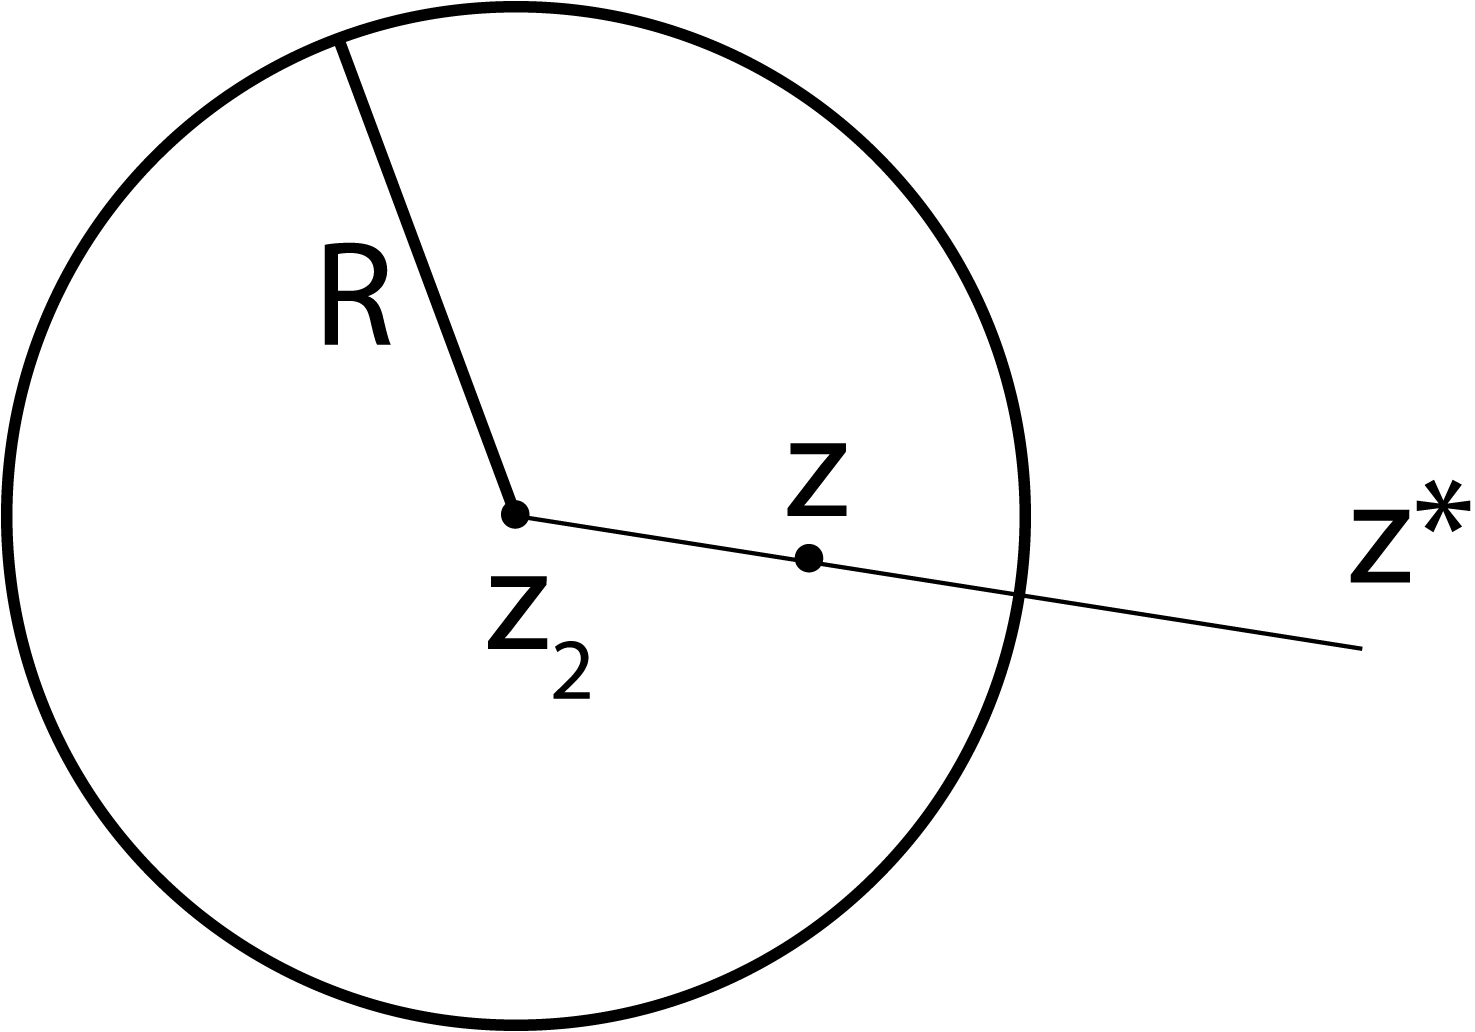
\includegraphics[width=5cm]{7_10}
	      \end{figure}
				\[\abs{z^* - z_0} \cdot \abs{z - z_0} = R^2\]
				\[z^* \text{ - симметрична } z \text{ отн окр. } \abs{z - z_0} = R\]
				Рассмотрим
	      \begin{figure}[H]
	        \centering
	        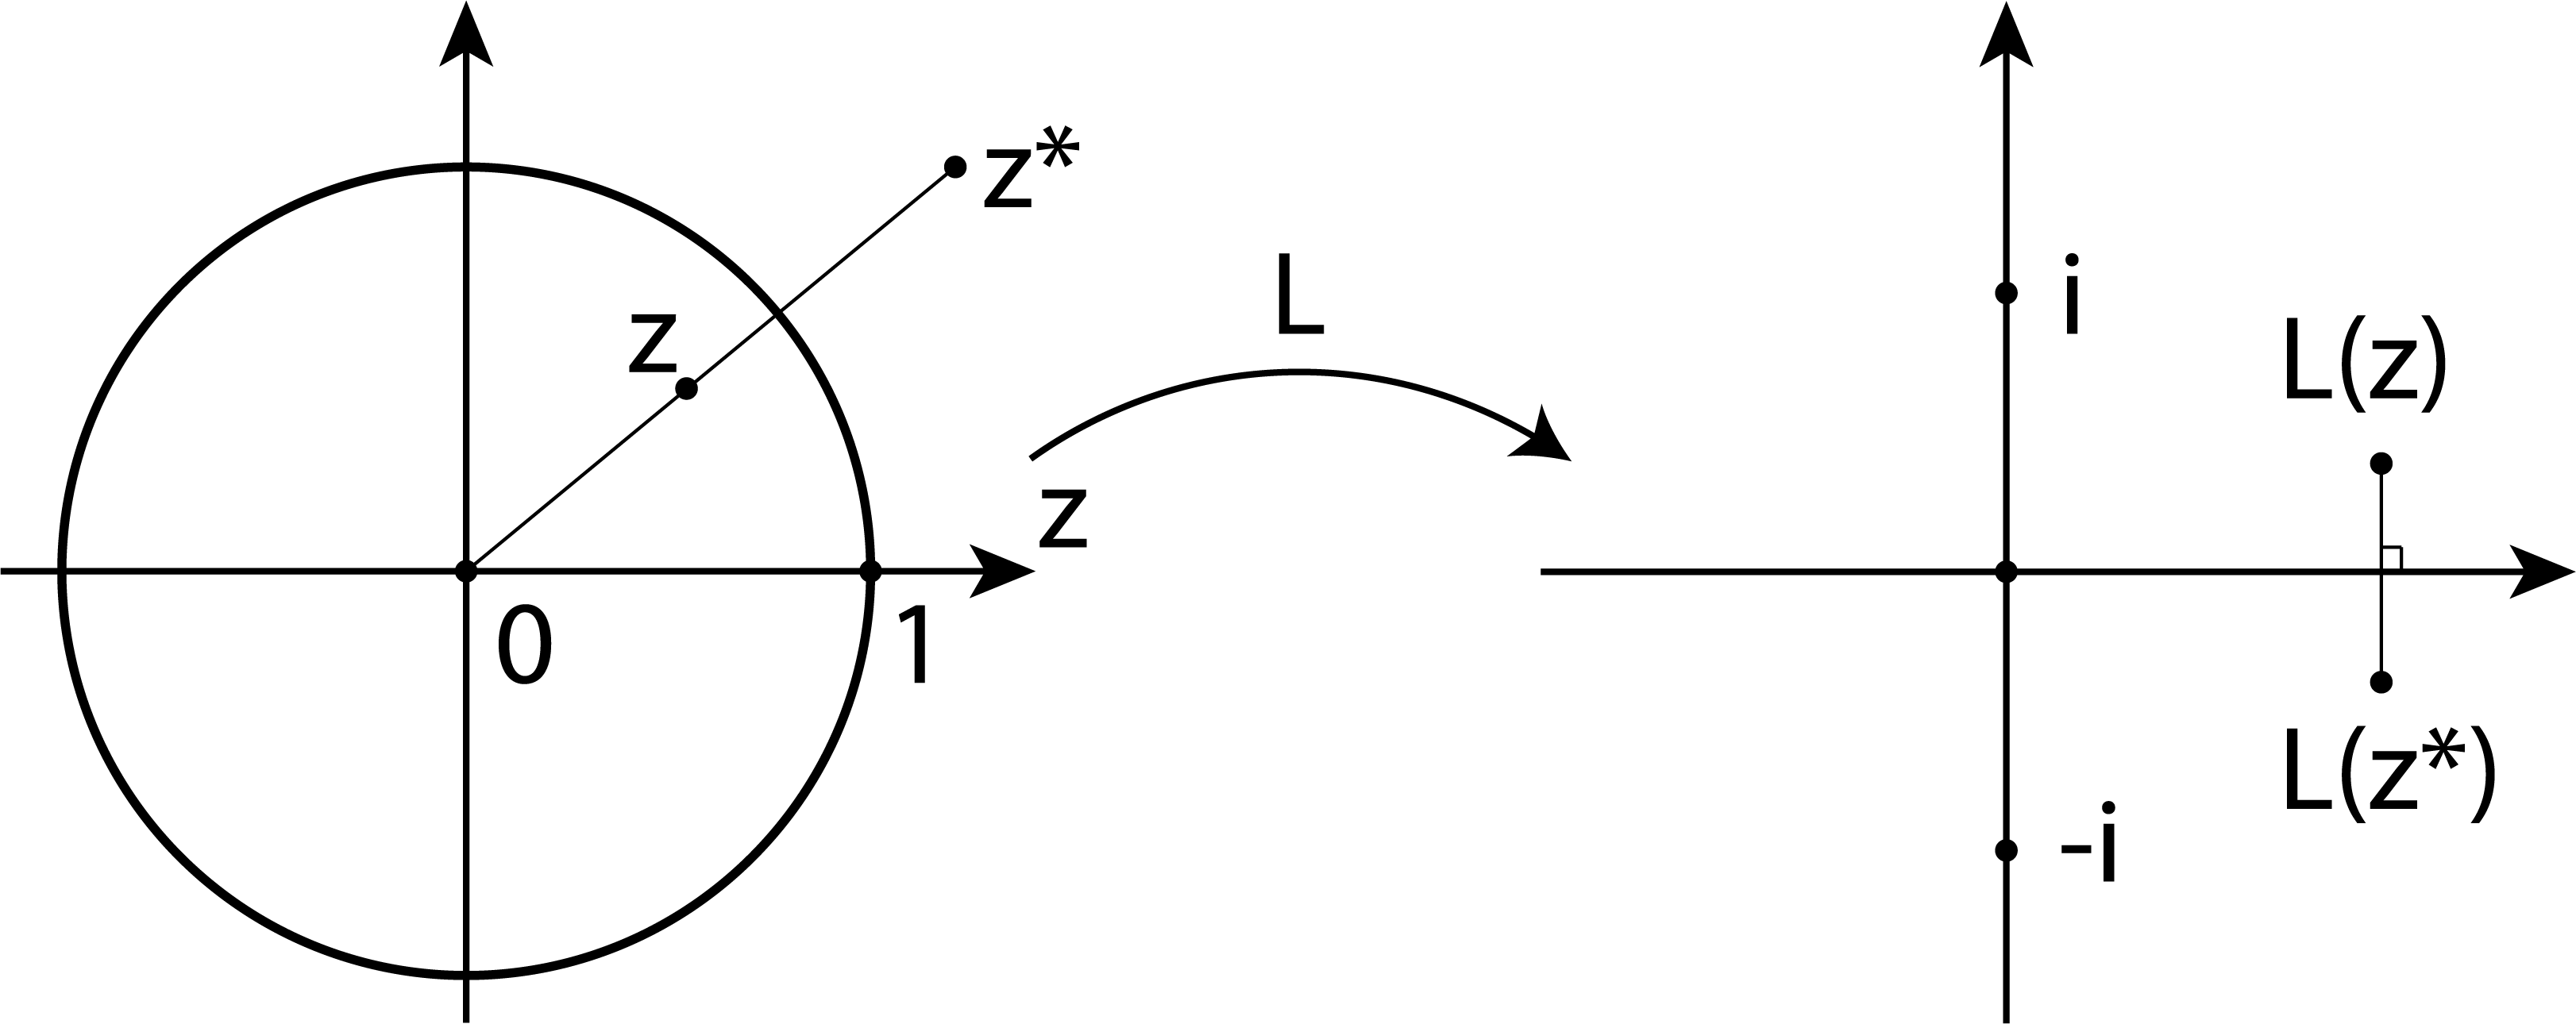
\includegraphics[width=8cm]{7_11}
	      \end{figure}
				\[z^* = \frac{1}{\abs{z}}(\cos \varphi + i \sin \varphi) =
				\frac{1}{\abs{z}} \cdot \frac{z}{\abs{z}}\]
				\[\begin{align}
					&L: & L(y) = \frac{z + b}{cz + d}\\
					&L(0) = i & L(0) = i = \frac{b}{d}\\
					&L(-1) = 0 & L(-1) = \frac{b - 1}{d - c} = 0\\
					&L(1) = \infty & L(1) = \frac{1 + b}{c + d} = \infty\\
				\end{align}\]
				\[b = 1 \qq d = -i \qq \frac{1 + 1}{c - i} = \infty \q c = i\]
				\[L(z) = \frac{z + 1}{iz - i} = -i \frac{z + 1}{z - 1}\]
				\[L(z) = -i \frac{z + 1}{z - 1} \]
				\[L(z^*) = -i \frac{\frac{z}{\abs{z}^2} + 1}{\frac{z}{\abs{z}^2} - 1} =
				-i \frac{z + \abs{z}^2}{z - \abs{z}^2}\]
				\[\overline{L(z)} = \overline{-i} \frac{(\overline{z} + 1) ^2 z}{(\overline{z} - 1)^2 z} =
				i \frac{\abs{z}^2 + z}{\abs{z}^2 - z} = L(z^*)\]
		\end{Definition}

		\begin{Example}
				\[7) \q f(z) = e^z = e^{x + iy} = e^x (\cos y + i\sin y) \text{ (по ф. Эйлера)}\]
				\[e^{iy} = \cos y + i \sin y \]
				\[e^{i\pi} = -1 \q  \text{ Замечательная формула, которая связывает 3 числа}\]
				\[(x, y) \os{e^z}{\to } (e^x \cos y;\ e^x \sin y)\]
	      \begin{figure}[H]
	        \centering
	        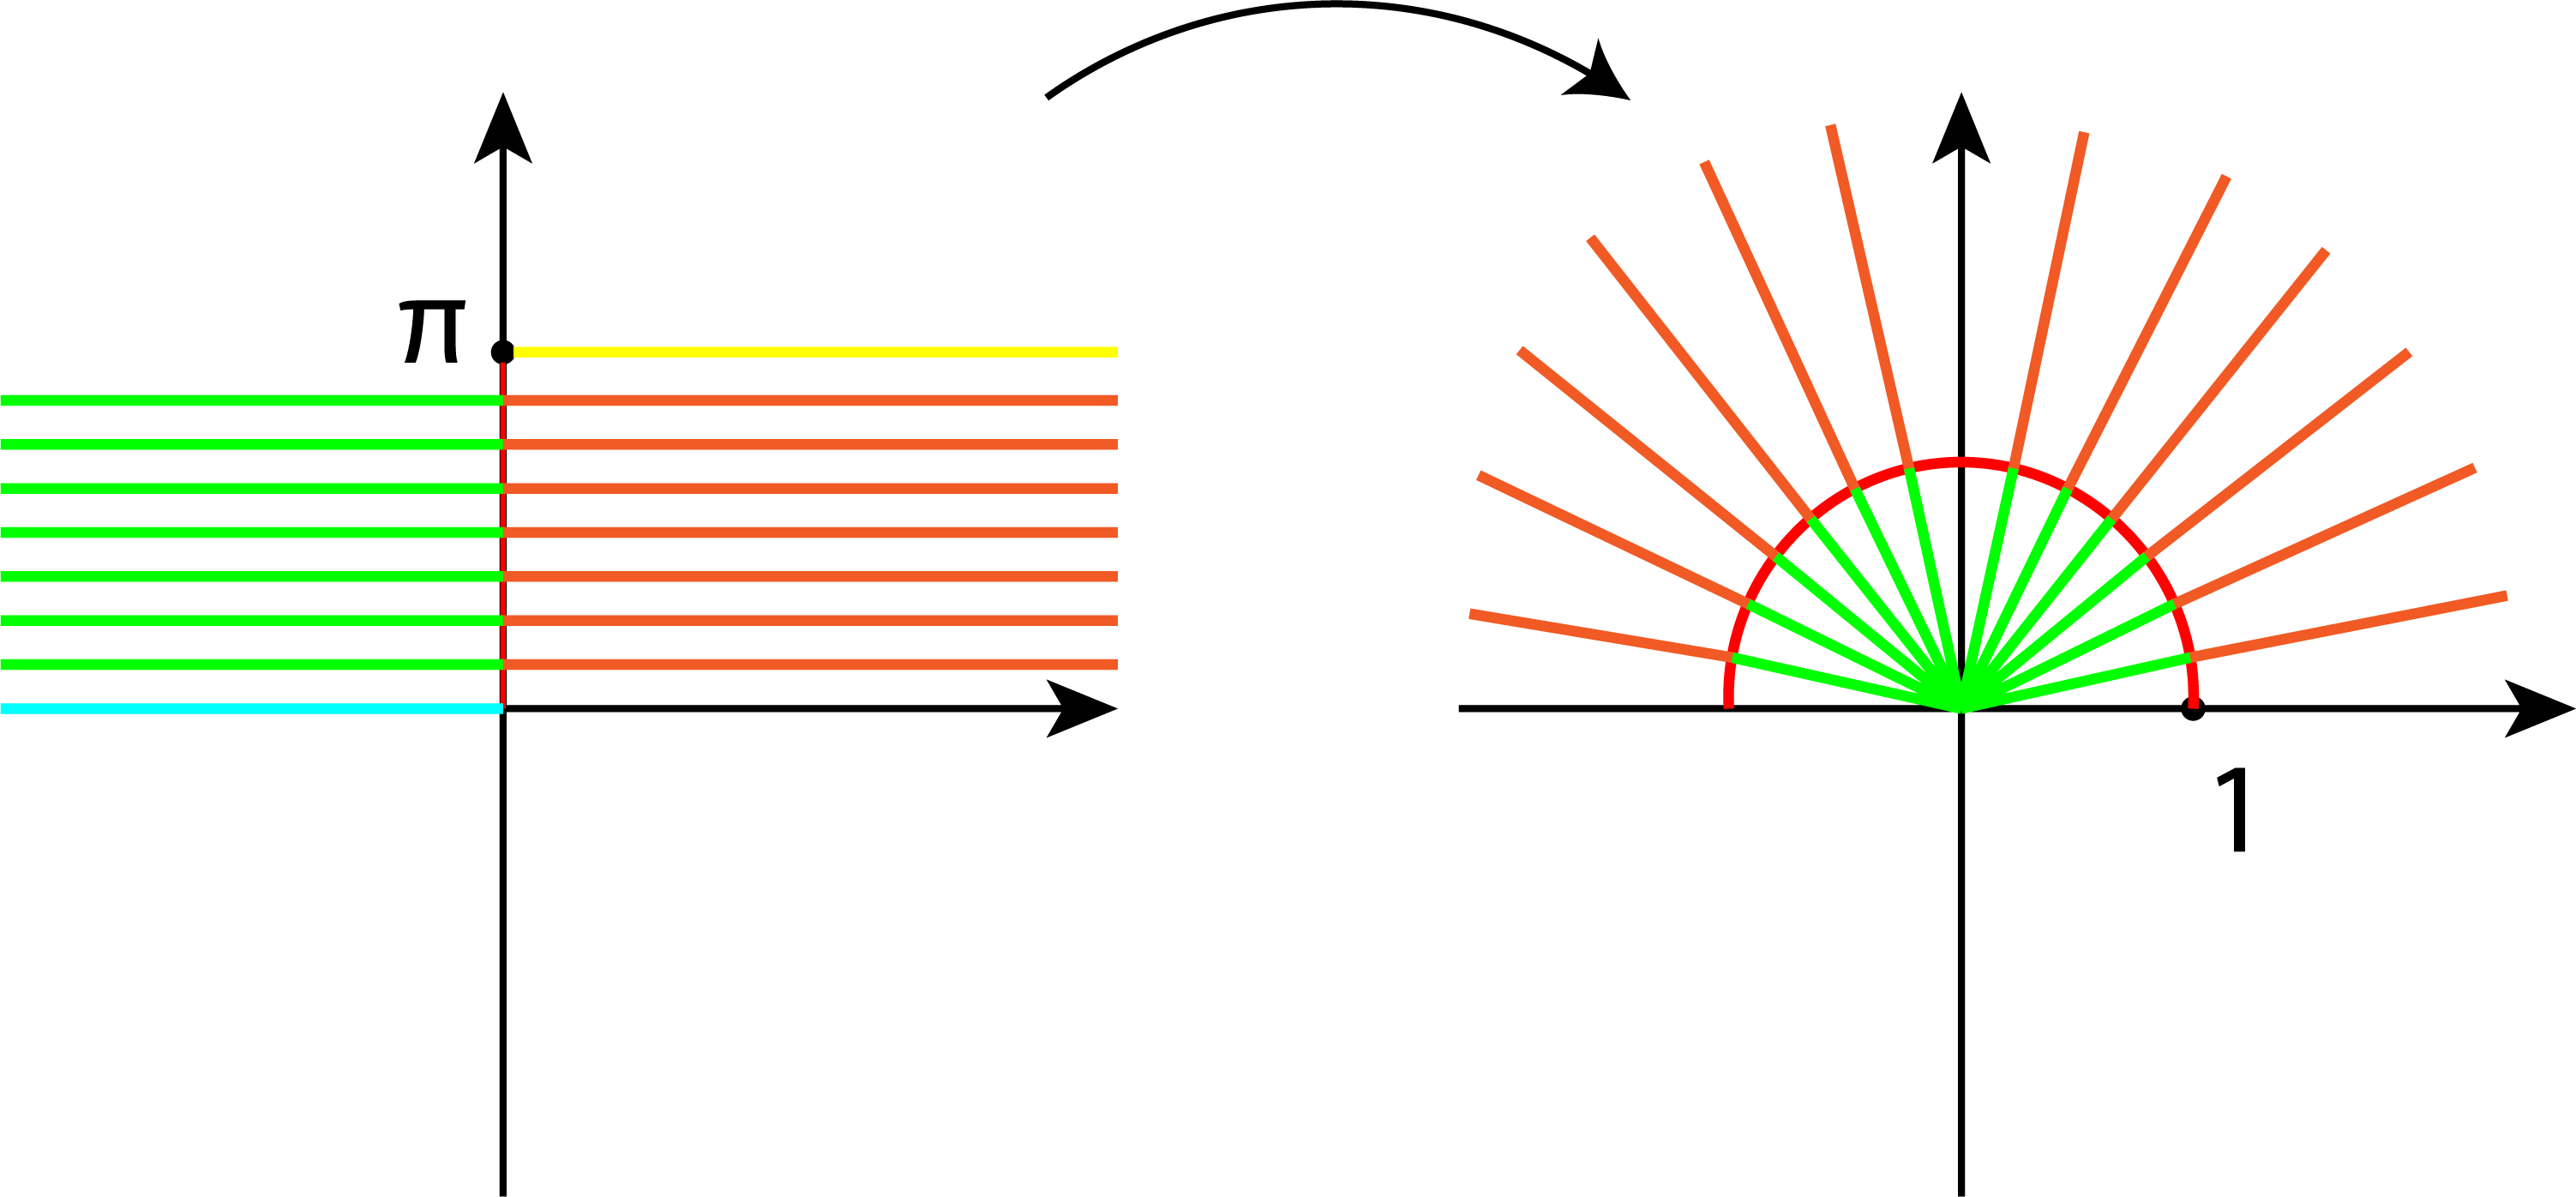
\includegraphics[width=8cm]{7_12}
	      \end{figure}
				\[\begin{cases}
					y = 0\\
					0 \leq x < \infty
				\end{cases} \os{e^z}{\to } e^x (\cos 0 + i \sin 0) = e^x \geq 1\]
				\[\begin{pmatrix}
					x = 0\\
					0 \leq y \leq \pi
				\end{pmatrix} \os{e^z}{\to } e^0 (\cos y + i\sin y)\]
				\[\begin{cases}
						y = \pi\\
						0 \leq x < +\infty
					\end{cases} \os{e^z}{\to} e^x (\underbracket{\cos \pi + i \sin \pi}_{-1}) = -e^x \leq -1\]
				hint: "для понимания можно представлять это как веер"
				\[e^z = e^x (\cos y + i \sin y) = e^x (\cos (y + 2 \pi k) + i \sin(y + 2 \pi k)) =\]
				\[ = e^{x + i(y + 2\pi k)} = e^{z + i \cdot 2 \pi k}  \]
				\[\text{Период } e^z \q T = e\pi k i\]
		\end{Example}
\end{lect}
\end{document}
